\documentclass{article}
\usepackage[utf8]{inputenc}
\usepackage{amsmath}
\usepackage{amsfonts}
\usepackage{enumitem}
\usepackage{amssymb} 
\usepackage{xcolor}
\usepackage{soul}
\usepackage{todonotes}
\usepackage[margin=2.5cm]{geometry}
\graphicspath{ {./images/} }

\title{Augmented Binary Search Trees}
\author{Jin Long Cao, Ethelia Choi}
\date{October 2022}

\begin{document}
\maketitle
\section*{Implementation of an Augmented BST}
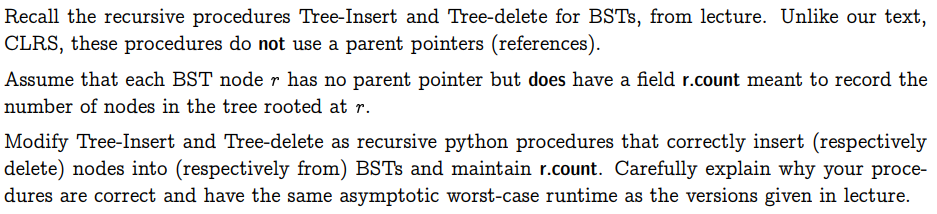
\includegraphics[width=\textwidth]{Binary Search Trees}
\section*{Solutions}
\subsection*{TREE-INSERT(root, x):}
\begin{enumerate}[itemsep=0pt,parsep=0pt]
    \item if root is NIL:  \quad\# x.key not already in S
    \item \qquad \# Found insertion point: create new node with empty children.
    \item \qquad root = TreeNode(x)
    \item \qquad root.count = 1
    \item elif x.key $<$ root.item.key:
    \item \qquad if TREE-SEARCH(root.left, x.key) is NIL: \quad\# NIL if x does not exist in the subtree.
    \item \qquad \qquad root.left.count += 1
    \item \qquad root.left = TREE-INSERT(root.left, x)
    \item elif x.key $>$ root.item.key:
    \item \qquad if TREE-SEARCH(root.right, x.key) is NIL: \quad\# NIL if x does not exist in the subtree.
    \item \qquad \qquad root.right.count += 1
    \item \qquad root.right = TREE-INSERT(root.right, x)
    \item else:  \quad\# x.key == root.item.key
    \item \qquad root.item = x  \quad\# just replace root's item with x
    \item return root
\end{enumerate}
Before inserting, assume count for all nodes are already maintain.\\~\\
\underline{Case 1:} Some element y in the tree has y.key = x.key, then we replace y with x and r.count does not change for any node. TREE-SEARCH will return y (which means it will not return NIL), therefore none of the counts (for any node) will increase (line 7 and 11). The function will recursively run (line 8 or 12) until it reaches to the y element then line 14 will run, replacing y with x.\\~\\
\underline{Case 2:} The element we're inserting does not exist in the tree already and is added as a leaf (line 1 to 4). All the ancestor of that leaf has their count increased by 1. TREE-SEARCH will return NIL, therefore anytime it recursively TREE-INSERT (line 8 or 12), it will increase the count by one for the parent node (line 7 and 11). Once it found it's insertion point, it will create a node and set that node's count to 1. \\~\\
In both cases, the TREE-SEARCH runtime will $O(\lg n)$ and the asymptotic worst-case runtime for this TREE-INSERT is $O(\lg n + \lg n) = O(2\cdot\lg n) = O(\lg n)$, which is the same as the versions given in lecture.

\begin{enumerate}[itemsep=0pt,parsep=0pt]
\subsection*{TREE-DELETE(root, x):}
    \item if root is NIL:  \# x.key not in S $--$ should not happen!
    \item \qquad pass  \# nothing to remove
    \item elif x.key $<$ root.item.key:
    \item \qquad if TREE-SEARCH(root.left, x.key) is not NIL: \quad\# NIL if x does not exist in the subtree.
    \item \qquad \qquad root.count -= 1
    \item \qquad root.left = TREE-DELETE(root.left, x)
    \item elif x.key $>$ root.item.key:
    \item \qquad if TREE-SEARCH(root.right, x.key) is not NIL: \quad\# NIL if x does not exist in the subtree.
    \item \qquad \qquad root.count -= 1
    \item \qquad root.right = TREE-DELETE(root.right, x)
    \item else:  \# x.key == root.item.key
    \item \qquad \# Remove root.item.
    \item \qquad if root.left is NIL:
    \item \qquad \qquad \# Missing left child (at least): replace with right child.
    \item \qquad \qquad \# descendants nodes' count don't change
    \item \qquad \qquad root.count = root.right.count
    \item \qquad \qquad root = root.right  \# NIL if both children missing
    \item \qquad elif root.right is NIL:
    \item \qquad \qquad \# Missing right child: replace with left child.
    \item \qquad \qquad \# descendants nodes' count don't change
    \item \qquad \qquad root.count = root.left.count
    \item \qquad \qquad root = root.left
    \item \qquad else:
    \item \qquad \qquad \# Root has two children: remove element with smallest key in
    \item \qquad \qquad \# right subtree and move it to root (replace root with successor).
    \item \qquad \qquad root.count = root.left.count + root.right.count
    \item \qquad \qquad root.item, root.right = TREE-DELETE-MIN(root.right)
    \item return root
\subsection*{TREE-DELETE-MIN(root):}
    \item \# Remove element with smallest key in root's subtree; return item and
    \item \# root of resulting subtree.
    \item if root.left is NIL:
    \item \qquad \# Root stores item with smallest key; replace it with right child. 
    \item \qquad return root.item, root.right
    \item else:
    \item \qquad \# Left subtree not empty: root not the smallest.
    \item \qquad root.count -= 1
    \item \qquad item, root.left = TREE-DELETE-MIN(root.left)
    \item \qquad return item, root
\end{enumerate}
\underline{Case 1:} TREE-DELETE is deleting an element that doesn't exist in the tree. This case should not happen (as stated in the pseudo-code) but should still be taken care of. Since the element does not exist in the tree, TREE-SEARCH will return NIL. If the element does not exist, it will recursively run (line 6 or 10) until "root is NIL" (line 1) and just pass. None of the counts (for any node) will change due to the fact that TREE-SEARCH is NIL (line 4 or 8).\\~\\
\underline{Case 2:} TREE-DELETE is deleting an element that does exist in the tree. TREE-SEARCH will not return NIL. Every ancestor of the element getting deleted will decrement their count by 1 and any descendants will keep the same count. The code will recursively run (line 6 or 10) and decrement the count for each ancestor (line 5 or 9) until it finds the element (line 11). Once the element is found, we replace it with one of their children (and their count) if the other one is NIL. If both children exist, we set the current node count to the sum of both children and find the successor to replace to it. Since the successor is replacing it, all ancestors of the successor node that is also a descendant of the deleted node will decrement their count (line 36).\\~\\
In both cases, the TREE-SEARCH runtime will $O(\lg n)$ and the asymptotic worst-case runtime for this TREE-DELETE is $O(\lg n+\lg n) = O(2\cdot\lg n) = O(\lg n)$, which is the same as the versions given in lecture.

\end{document}